%%%%%%%%%%%%%%%%%%%%%%%%%%%%%%%%%%%%%%%%%%%%%%%%%%%%%%%%%%%%%%%%%%%%%%%%%%
\section{Hieroglyphs}
\index{Hieroglyphen}
%%%%%%%%%%%%%%%%%%%%%%%%%%%%%%%%%%%%%%%%%%%%%%%%%%%%%%%%%%%%%%%%%%%%%%%%%%
%

The standard for writing texts in \textit{toki pona} is the Latin alphabet.
However, writing systems based on hieroglyphics were also developed.
Depending on the system, the symbols represent letters, syllables or words.
A system that uses a symbol for each word is \textit{sitelen pona} \cite{www:tokipona.org:02}.
Jonathan Gabel has developed a very nice hieroglyphic script.
\textit{sitelen sitelen} \cite{www:jonathangabel.com:01} looks similar to Mayan hieroglyphics.

Unfortunately, most of these systems has not punctuation marks or special characters.
A system that also has symbols for punctuation marks is \textit{sitelen pona pi jan Makuwe} \cite{www:janMakuwe:01}.
This hieroglyphic script represents syllables.
% Vowels are written as diacritics on the consonants they follow.
% To write an "n" at the end of a syllable, write a circle in the center of the symbol.

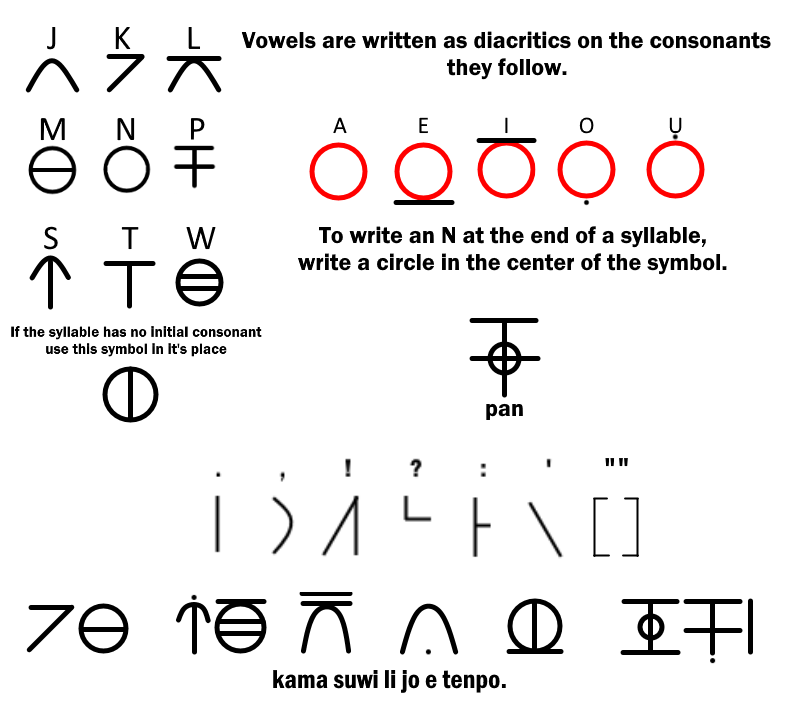
\includegraphics[scale=0.5]{sitelen_pona_pi_jan_Makuwe}

%
%%%%%%%%%%%%%%%%%%%%%%%%%%%%%%%%%%%%%%%%%%%%%%%%%%%%%%%%%%%%%%%%%%%%%%%%%%
% eof
